\begin{exo}
  \donnee{La durée de vie en heures d'un certain composant électronique peut être modélisée par une variable aléatoire X dont la fonction de densité est donnée par $ f_x(u) =
  	\begin{cases}
  		\frac{c}{u^2} & \text{si $ 10 < u < 20$ } \\
  		x & \text{$0$ sinon.} \\
  	\end{cases}$
  }
	\begin{subexo}{Calculez la constante $c$.}
		\begin{center}
			Calculons l'intégrale de la fonction de densité de 10 à 20: 
		\end{center}
		\begin{align*}
			\displaystyle\int_{10}^{20}{\frac{c}{u^2}}du &= \frac{-c}{u}\bigg\vert_{10}^{20}\\
			&= \frac{-c}{20} + \frac{c}{10} \\
			&= \frac{c}{20}
		\end{align*}
		\begin{center}
			Nous avons $\displaystyle\int_{-\infty}^{\infty}{f_x(u)}du = 1$. \\ Comme, $\displaystyle\int_{-\infty}^{\infty}{f_x(u)}du = \displaystyle\int_{10}^{20}{\dfrac{c}{u^2}}du \iff 1 = \frac{c}{20}$ \\
			Finalement, $c=20$
		\end{center}
	\end{subexo}
	\begin{subexo}{Déterminez la fonction de répartition de X et tracer son graphe.}
		\begin{center}
			Il faut séparer trois cas : 
		\end{center}
		\begin{align*}
			&1) x \in \intervalleoo{-\infty}{10} \\
			&2) x \in \intervalleff{10}{20} \\
			&3) x \in \intervalleoo{-\infty}{10} \\
		\end{align*}
		\begin{center}
			Prenons le deuxième cas,
		\end{center}
		\begin{align*}
			P(X \leq x) = F_x(x) &= \int_{-\infty}^{x}{f_x(u)}du \\
			&= \displaystyle\int_{10}^{x}{\frac{c}{u^2}}du \\
			&= \frac{-c}{u}\bigg\vert_{0}^{x} \\
			&= \frac{-c}{x} + \frac{c}{10} \\
			&= \frac{-20}{x} + 2 \\
		\end{align*}
		\begin{center}
			Finalement,   	$ F_x(x) =\begin{cases}
				0 & \text{si $x \le 10$} \\
				\frac{-20}{x} + 2 & \text{si $10 \leq x \leq 20$} \\
				1 & \text{si $x \geq 20$} \\
			\end{cases}$
		\end{center}
		\begin{center}
			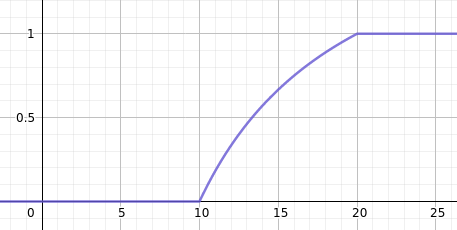
\includegraphics[width=10cm]{ex3_b.png}
		\end{center}
	\end{subexo}
	\begin{subexo}{Calculez la probabilité $P(X > 15)$.}
		\begin{align*}
			P(X > 15) &= \displaystyle\int_{15}^{20}{\frac{c}{u^2}}du \\
			&= F_x(20) - F_x(15) \\
			&= \left( \frac{-20}{20} + 2 - \left(\frac{-20}{15} + 2\right)\right) \\
			&= -1 + \frac{4}{3} \\ 
			&= \frac{1}{3}
		\end{align*}
		\begin{flushleft}
			Deuxième manière,
		\end{flushleft}
		\begin{align*}
			P(X > 15) &= 1 - P(X \leq 15) \\
			&= 1 - \displaystyle\int_{10}^{15}{\frac{c}{u^2}}du \\
			&= 1 - (F_x(15) - F_x(10)) \\
			&= 1 - \left( \frac{-20}{15} + 2 - \left(\frac{-20}{10} + 2\right)\right) \\
			&= 1 - \left(2 -\frac{4}{3}\right) \\
			&= \frac{1}{3}
		\end{align*}
	\end{subexo}
	\begin{subexo}{Calculez la durée de vie espérée d'un composant électronique de ce type.}
		\begin{center}
			Il s'agit de calculer l'espérance. Par définition, elle est définie comme : $E(x) = \displaystyle\int_{-\infty}^{\infty}{u\cdot f(u)}du$
		\end{center}
		\begin{align*}
			E(x) &= \displaystyle\int_{-\infty}^{\infty}{u\cdot f(u)}du \\
			&= \displaystyle\int_{10}^{20}{u \cdot \frac{c}{u^2}}du \\ 
			&= \displaystyle\int_{10}^{20}{\frac{c}{u}}du \\ 
			&= c\cdot \ln{u}\bigg\vert_{10}^{20} \\
			&= c \cdot (\ln{20} - \ln{10}) \\
			&= 20 \cdot \ln{2}
		\end{align*}
	\end{subexo}
\end{exo}
